\section{Ausgangslage}
Hier werden das Arbeitsumfeld und die Aufgaben beschrieben, aus denen sich die Problemstellung dieser Semesterarbeit ergeben hat.

\subsection{swisstopo bei AWS}
Es liegt auf der Hand, dass die swisstopo in ihrer Rolle als \emph{Geoinformationszentrum} auf Cloud Computing setzt. Die swisstopo nutzt Cloud Computing mit AWS\footnote{Amazon Web Services} seit mehr als 10 Jahren für den Betrieb des Geoportal des Bundes.
 
\textit{"Mit der BGDI\footnote{Bundesgeodateninfrastruktur: Viewer und andere Services.} unter AWS können wir derzeit ca. eine Million Internetbenutzer pro Monat bedienen. Dank AWS können wir die zur Zuordnung neuer Server benötigte Zeit erheblich verkürzen und unseren Fokus auf echte Kundenanforderungen verstärken."} \cite{Christ2020}.


\subsection{Publikation von Geodaten}
Wie bereits erwähnt, können auf dem Viewer ca. 800 Themen wie Wanderwege, Solarkataster und Luftfahrthindernisse angesehen werden. Unser Team publiziert diese Daten. Der Nachführungszyklus wie auch der Aufwand zur
Aufbereitung der Daten fürs Web sind unterschiedlich. Einige Daten werden manuell aufwändig aufbereitet, andere
stündlich automatisch nachgeführt.

\subsection{Web-Services}
Nebst der Publikation der Daten ist unser Team für den Betrieb und der Weiterentwicklung der Web-Services
und des Viewers verantwortlich. Der ganze Technologie Stack wurde schon länger nicht mehr grundlegend erneuert. Zurzeit wird
die gesamte Architektur analysiert und überarbeitet, um eine gestaffelte Migration auf eine neue
Lösung zu ermöglichen.
Einige Rahmenbedingungen dieser zukünftigen Architektur sind bereits klar: Das Geoportal des
Bundes wird weiterhin in der AWS Cloud betrieben werden, die Migration wird vor allem über
Microservices gestaffelt erfolgen, diese Services werden als Docker Container laufen, Amazon
Elsatic Kubernetes Service wird die Orchestrierung der Container übernehmen; und für Continuous
Integration wird AWS Codebuild/Pipeline zum Einsatz kommen.

\newpage

\subsection{Exkurs 3D Daten}
Die swisstopo erfasst und aktualisiert Daten mit einem räumlichen Bezug. Diese Geodaten sind die Basis für die Ableitung in eine Vielzahl von Produkten, wie die Landeskarten 1:25'000. Nebst Karten gibt es die Produktpalette der Landschaftsmodelle. Diese geben die Objekte der Landschaft im flexiblen Vektorformat wieder. Sie bestehen aus thematischen Ebenen (Bsp. Gebäude). Jede Ebene umfasst georeferenzierte Punkt-, Linien-, Flächen- oder 3D-Objekte. Jedes Objekt enthält Attribute und Beziehungen \cite{toposhop2010}.

Zu den Lanschaftsmodellen gehören Produkte wie swissTLM3D und swissBuildings3D. Im Viewer wird eine Auswahl von Themen aus eben diesen Landschaftsmodellen dargestellt: Zurzeit Gebäude, Bäume, Seilbahnen, Namen und das Terrain. Vor wenigen Jahren wurden diese 3D Daten mit einem grossen Effort medienwirksam publiziert.

\begin{figure}[H]
	\centering
	\href{https://s.geo.admin.ch/8a8ce63073}{
	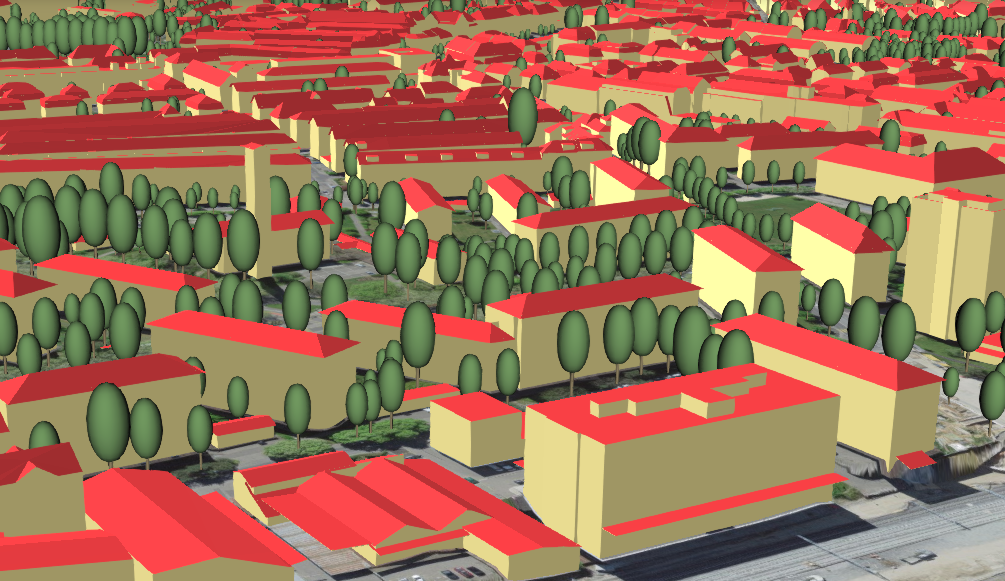
\includegraphics[width=.80\textwidth]{bfh_3d}}
	\caption{Im Viewer werden zurzeit Gebäude, Bäume, Seilbahnen, Namen und das Terrain dargestellt. Um aktuell zu bleiben, müssen diese 3D Daten regelmässig nachgeführt werden.}
	\label{fig:bfh_3d}
\end{figure}

Seit der Erstpublikation ist inzwischen etwas Zeit vergangen. Als die ersten Aktualisierungen der Daten anstanden, wurde den Beteiligten bewusst, dass sich diese nicht einfach so \emph{auf Knopfdruck} realisieren lässt: Seit der Erstpublikation hat es personelle Wechsel gegeben und punkto Dokumentation und Automatisierungsgrad wurden Lücken identifiziert.

Es gibt immer gute Gründe für \emph{technische Schulden}, wie in diesem Fall für positive medienwirksame Reaktionen\footnote{Wie Bsp. auf watson.ch oder Twitter \cite{watson2018}}. Früher oder später müssen diese abgebaut werden, weil es einen direkten Einfluss auf die Wartbarkeit des Produktes hat \cite{technischeschulden2010}.

\section{Der Use Case}
\subsection{Problemstellung}
Es ist der swisstopo schon lange ein Anliegen, dass die Publikationvorgänge von Geodaten optimiert werden
sollen. Wann immer möglich, soll der Automatisierungsgrad erhöht werden.

Besonders aufwändig erweist sich zurzeit die Publikation von 3D Daten. Die manuelle Publikation
der 3D Daten benötigt eigene Tools, die auf einem performanten und somit teuren Rechner laufen
müssen. Ausserdem erfordert die Bereitstellung einen hohen Koordinationsaufwand zwischen der
Infrastruktur und der Entwicklung. Dabei passiert es, dass Mängel in den 3D Daten erst nach
beendeter Webpublikation bemerkt werden; und der ganze Publikationsvorgang muss wieder von
vorne gestartet werden.
Auch dem Hersteller der 3D Daten (dem Bereich Topografie) wäre es ein Anliegen, wenn er diese
Daten selbst automatisch publizieren und prüfen könnte.

Einerseits soll in dieser Arbeit mittels POC\footnote{Prove of Concept} aufgezeigt werden, wie der Automatisierungsgrad erhöht werden könnte. Andererseits soll untersucht werden, ob für die Verarbeitung Budget Instanzen\footnote{Amazon Spot Instanzen} anstelle von On-Demand Instanzen\footnote{Herkömmliche EC2 Instanzen.} verwendet werden können und wie deren Einsatz aussehen könnte.

\subsubsection{Budget Instanzen}
Amazon preist Budget Instanzen folgendermassen an: \textit{"Mit Amazon EC2 Spot-Instances können Sie die Vorteile nicht genutzter EC2-Kapazitäten in der AWS Cloud nutzen. Spot-Instances sind mit einem Rabatt von bis zu\\ 90 \% im Vergleich zum On-Demand-Preis verfügbar. Sie können Spot-Instances für diverse statuslose, fehlertolerante und flexible Anwendungen verwenden. Dazu zählen unter anderem Big-Data-Anwendungen, auf Containern ausgeführte Workloads, CI/CD, Webserver-Anwendungen, HPC-Anwendungen (High-Performance Computing) sowie Test- und Entwicklungs-Workloads."} \cite{AmazonAWSSpot:1}.


\begin{figure}[H]
	\centering
	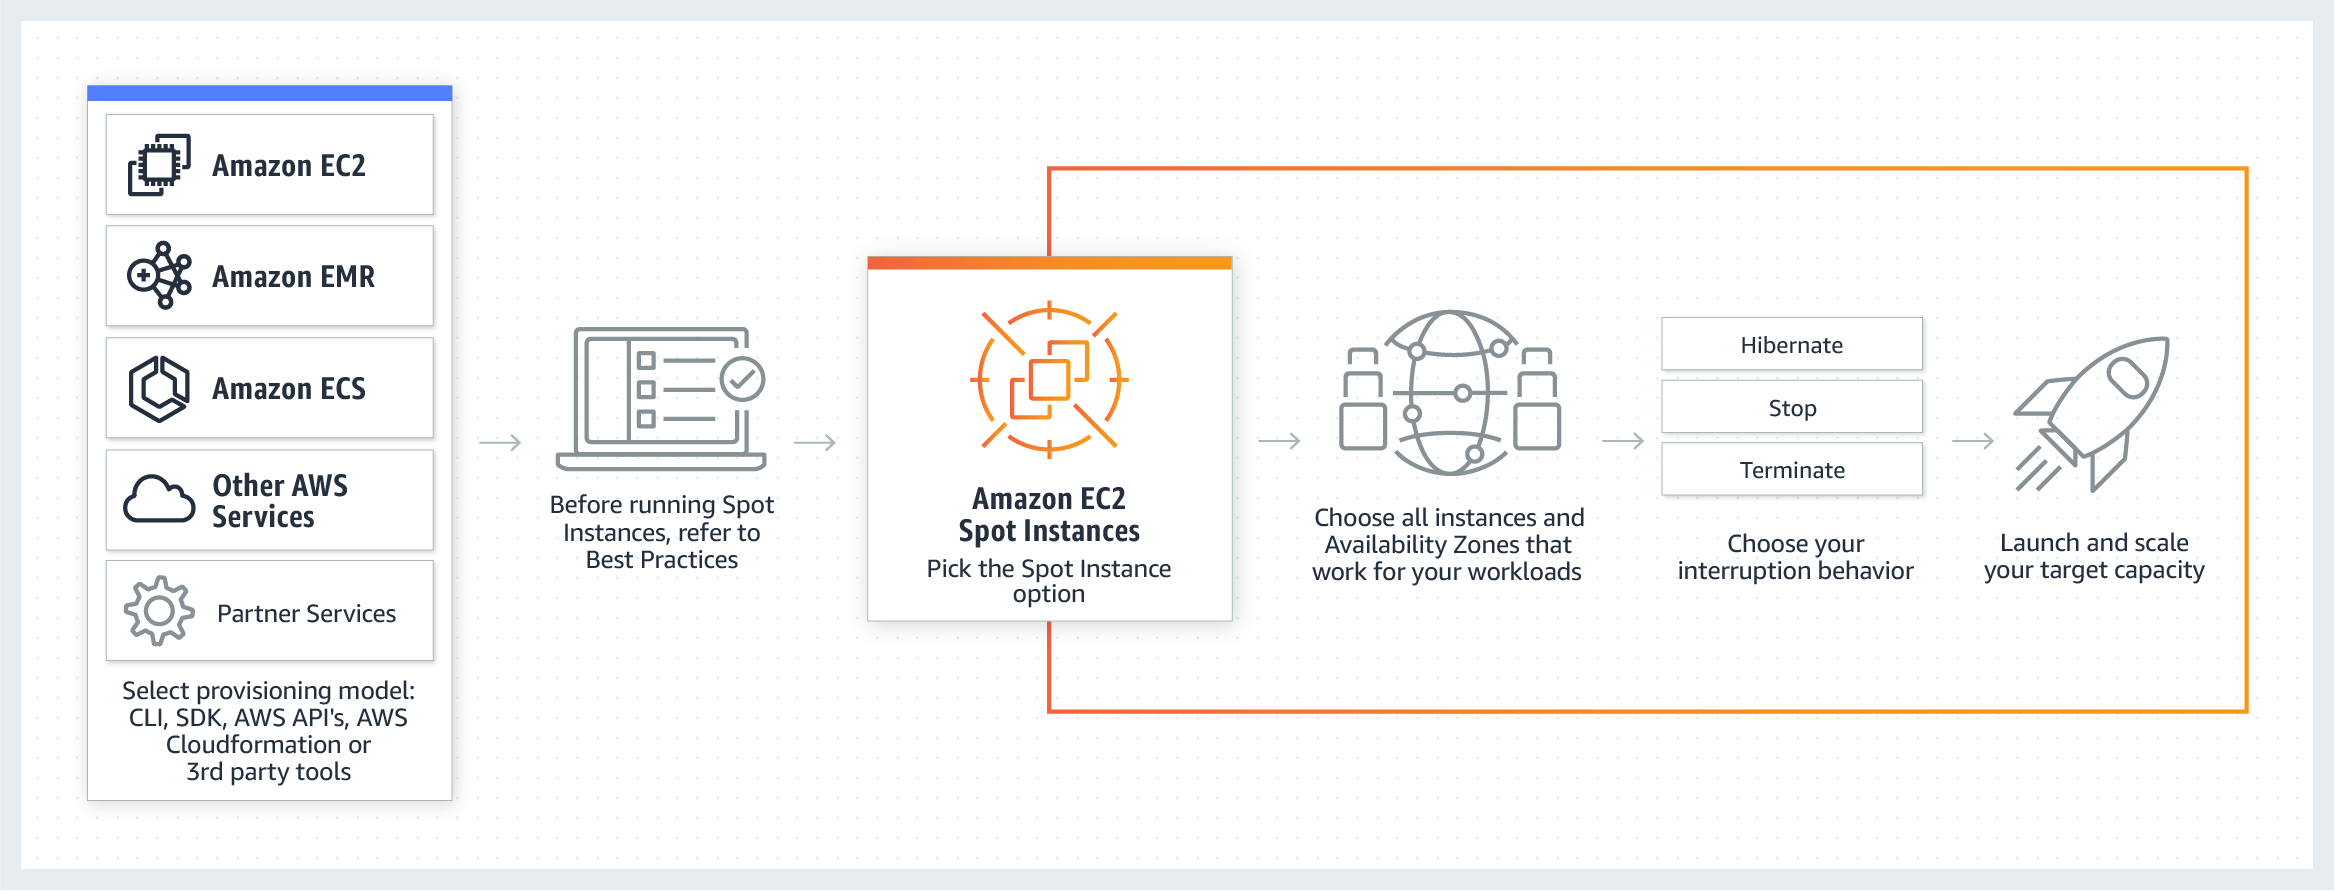
\includegraphics[width=.70\textwidth]{spot}
	\caption{So funktioniert das Ausleihen von Bugdet (SPOT) Instanzen}
	\label{fig:spot}
\end{figure}

Das Verkaufsargument \emph{90 \%} Rabatt ist eine Ansage: Eine Preis-Aktion, ein Budget Produkt, damit AWS nicht genutzte EC2-Kapazitäten doch noch verkaufen kann. Der Konsument gibt viel weniger aus, mit dem Hacken, dass einem die Instanz innerhalb von 2 minütiger Vorankündigung weggenommen werden kann.

Möchte man die EC2 Spot Instanzen für die Geodatenverarbeitung einsetzen, muss also ein Weg gefunden werden, um mit diesen Unterbrüchen umgehen zu können.

Wie auf der Abbildung \ref{fig:spot} dargestellt, kann das Verhalten der Instanz bei einem Interrupt\footnote{Wenn Amazon die Spot Instanz für einen anderen Zweck beanspruchen möchte, die wegnimmt.} definiert werden. Es besteht dabei sogar die Möglichkeit eines \emph{Hibernate}, dass der Zustand des RAMs auf der Festplatte persistiert wird.

Diese 2 minütige Vorankündigung eines Intterupts kann auch via RESTful Abfrage\footnote{EC2 Spot Instance Interruption Notice, eine HTTP Abfrage: Im Anhang \ref{appendix:restful} hat es ein Beispiel dazu.} von der Instanz aus abgefragt werden.

Diese Vorankündigung lässt sich auch via AWS CLI abfragen. In einem grösseren Setup könnte das Signal der Vorankündigung auch mit dem AWS Überwachungstool \emph{CloudWatch} verarbeitet werden.


\subsection{Ist-Zustand der 3D Datenpublikation}
\subsubsection{Prozess der Publikation}
Das Aufzeigen des Ist-Zustandes der 3D Datenpublikation soll helfen sich einen Überblick, eine Ausgangslage, zu verschaffen. Es bildet die Grundlage, um die Frage zu beantworten, welche Arbeiten erledigt werden müssen, um die 3D Daten im Web zu publizieren? Welche Arbeitsschritte könnten automatisiert werden? 

Eine Datenpublikation läuft folgendermassen ab: Sobald der Auftrag für eine 3D Datenpublikation erteilt wurde\footnote{Vom Bereich Topografie}, müssen zurzeit folgende Schritte, die in der Abbildung \ref{fig:ist_zustand} referenziert sind, erledigt werden:

\begin{figure}[H]
	\centering
	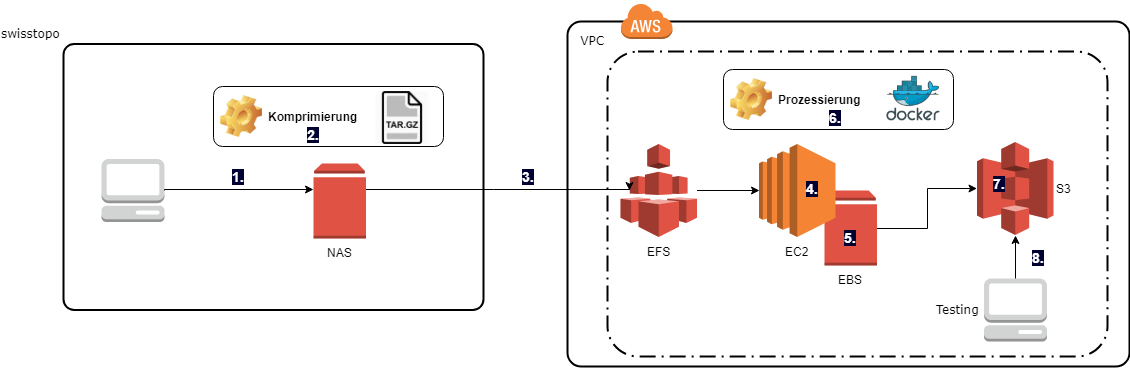
\includegraphics[width=.90\textwidth]{ist_zustand}
	\caption{Arbeitsschritte, die es braucht, um die 3D Daten zu Publizieren.}
	\label{fig:ist_zustand}
\end{figure}

\begin{enumerate}
\item Die Rohdaten\footnote{Das Format der Rohdaten ist KML/COLLADA} werden vom Auftraggeber (Bereich Topografie) auf einem NAS bereitgestellt.
\item Da es sich um Millionen Dateien handelt, werden diese je Kartenblatt erst einmal gezippt, um so (weil bedeutend weniger Dateien) schneller kopiert werden zu können.
\item Kopieren der gezippten Dateien vom swisstopo Netzwerk in die Amazon Cloud (AWS VPC\footnote{AWS: Amazon Web Services, VPC: Virtual Private Network. Ein Kopieren}) kopiert\footnote{Via \emph{rsync}}
\item Parallel dazu wird die IT via Ticket gebeten einen Server mit dem entsprechenden Image\footnote{Eine EC2 Instanz \emph{eine m4.10xlarge} aus einem bereits vorhandenes AMI} bereitzustellen.
\item Kopieren und Entzippen der Rodaten auf die gemountete Festplatte\footnote{Ein EBS Volume} des Servers.
\item Die Daten auf dem Server via Docker verarbeiten\footnote{Umwandeln ist das Web-Format \emph{Cesium3DTiles}}.
\item Kopieren der Web-optimierten Daten auf S3.
\item Die Daten visualisieren, um inhaltlich testen zu können. Ein Codepen Projekt\footnote{SaaS: Eine Webseite, um Front-End Code zu schreiben, zu testen, und bereitzustellen (\href{https://codepen.io}{codepen.io})}, dass auf die 3D Tiles zugreift.
\end{enumerate}

\subsubsection{Aufwand der Verarbeitung}
\label{aufwand_prozessierung}
Folgende Schritte sind besonders aufwendig:
\begin{itemize}
\item \textbf{Abb. \ref{fig:ist_zustand}, Schritt 2. und 5.}: Das Kopieren / Zippen (Packen und Entpacken) der Rohdaten nimmt lange.
\item Es kommt immer mal wieder vor, dass Daten korrupt sind, was zu einer Nachlieferung führt, mit der Gefahr, dass es mit Versionen der Lieferung zu einem Durcheinander kommen könnte.
\item \textbf{Abb. \ref{fig:ist_zustand}, Schritt 4.}:Unsere IT muss für die Verarbeitung eine EC2 Instanz mit EFS bereitzustellen. Um laufende Kosten zu verringern, wird diese Instanz nach getaner Arbeit\footnote{Der Verarbeitung.} wieder gestoppt. Falls mit den Daten etwas nicht in Ordnung ist, muss dieser Schritt von der IT wiederholt werden. Nebst der Bemühung der IT, muss auf der Instanz selber anschliessend das eine und andere manuell installiert und konfiguriert werden.
\end{itemize}

\subsubsection{Technische Komponenten}
Auflistung der technischen Komponenten:
\begin{itemize}
\item \textbf{Abb. \ref{fig:ist_zustand}, Schritt 2., 3. und 5.}: Das Komprimieren und Kopieren der Rohdaten erfolgt mit Linux Bordmitteln (\emph{cp}, \emph{rsync}, \emph{tar})
\item \textbf{Abb. \ref{fig:ist_zustand}, Schritt 4. und 7.}: Erfolgen via AWS CLI
\item \textbf{Abb. \ref{fig:ist_zustand}, Schritt 6.}: Via Docker. Der Container wurde von der Firma Analytical Graphics Inc. \cite{AGI2010} bereitgestellt. Das Tool, das die Rohdaten in ein Web-Format umwandelt, wird mit Node.js ausgeführt.
\item \textbf{Abb. \ref{fig:ist_zustand}, Schritt 7.}: Ein Projekt, um die Daten im Browser betrachten und inhaltlich Testen zu können, erfolgt über die Webseite codepen.io.
\end{itemize}


